\documentclass[journal]{vgtc}
\usepackage[utf8]{inputenc}
\usepackage{geometry}
\usepackage{fullpage}
\usepackage{natbib}
\usepackage{adjustbox}
\usepackage{graphicx}
\usepackage{balance}
\usepackage{url}

\title{TraViz: Visualization of Traces in Distributed Systems}
\author{Vaastav Anand and Matheus Stolet}

\abstract{
    In this work we present TraViz, an interactive visualization tool for exploring and analysing 
    distributed traces to troubleshoot and debug performance problems in distributed systems.
    Through the use of composite filtering of multiple dimensions of the dataset, TraViz
    provides developers an easy to use way to find outlier traces. With TraViz's traceview
    swimlane idiom, the users can drill down into a single trace to analyze the trace
    for performance issues at the detail level of an operating system thread. TraViz's
    comparison idiom allows users to compare the Graphical structure of 2 traces of interest
    to highlight the key differences between the traces.
    The aggregation idiom allows users to find uncommon occuring events across traces by
    constructing a luminance coded super graph of all the distributed traces.
    Additionally, TraViz is the first visualization tool that provides an integrated view
    of the static source code of the system with dynamic information collected about the
    system via distributed traces which can help the users in identifying locations in the
    source code that would be ideal for performance optimizations.
}

\keywords{Distributed Tracing, Graph Comaprison, Graph Aggregation, Source Code Integration}

\teaser{
    \centering
    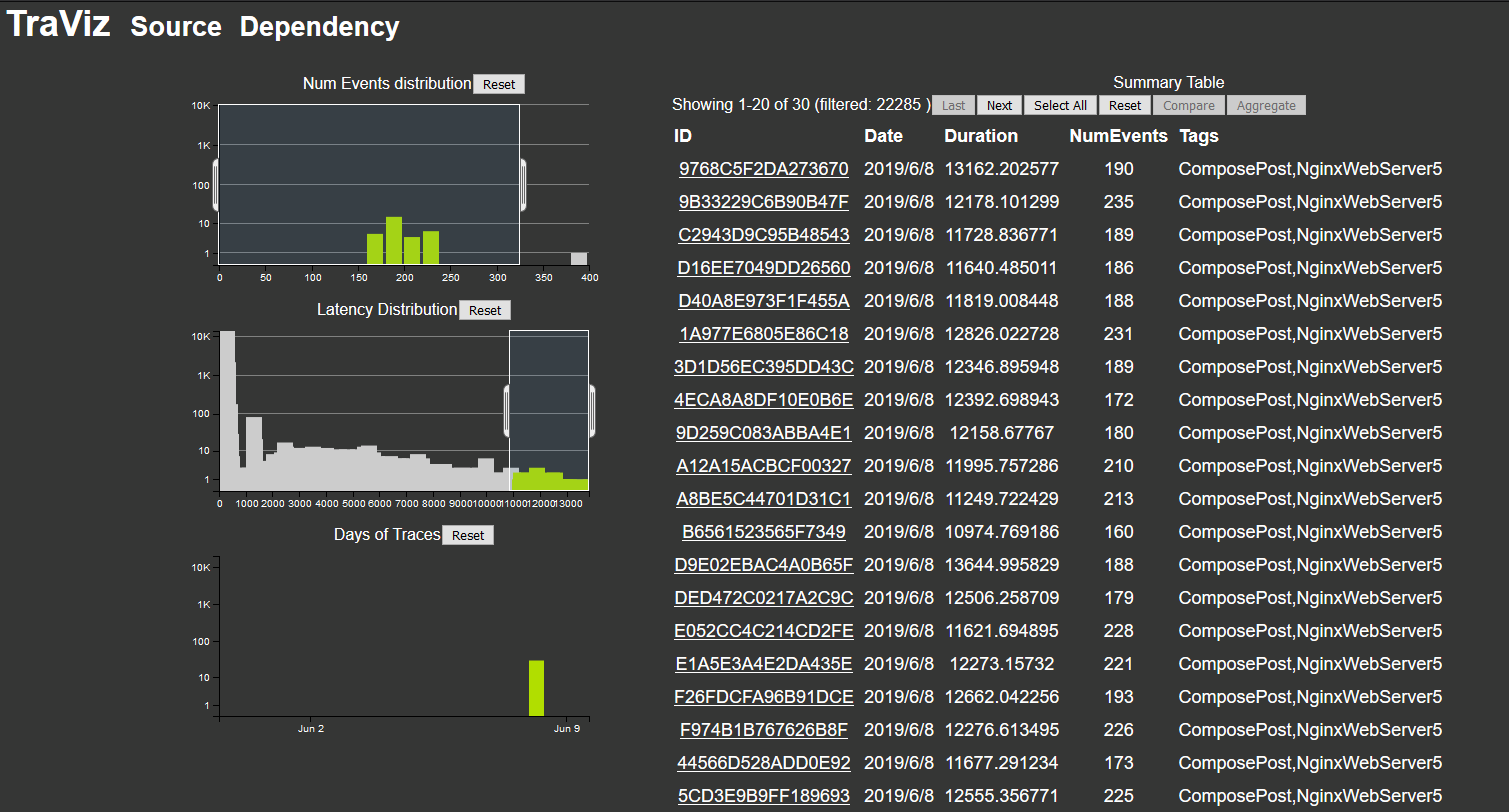
\includegraphics[width=\linewidth]{fig/crossfilter}
    \caption{TraViz overview layout, showing a filtered selection of distributed traces using filters on distributions of multiple dimensions of the distributed traces dataset.}
      \label{fig:teaser}
}

\date{}

\vgtcinsertpkg

\begin{document}

\maketitle

\section{Introduction}

Distributed systems are prevalent in society to the extent that billions of people either directly or 
indirectly depend on the correct functioning of a distributed system. From banking applications to social
networks, from large-scale data analytics to online video streaming, from web searches to cryptocurrencies,
most of the successful computing applications of today are powered by distributed systems.
The meteoric rise of cloud computing in the past decade has only increased our dependence on these
distributed systems in our lives.

Tasks like monitoring, root cause analysis, performance comprehension require techniques that cut across component,
system, and machine boundaries to collect, correlate, and integrate data. Distributed Tracing is one such cross-cutting technique
that correlates events across the system to a specific request by propagating a unique context per system with the request.
A trace represents the path of one request through the system and contains information such as the timing of requests, 
the events executed, and the nodes where these events were executed. Moreover, traces can be used
to identify slow requests and understand the difference between request executions. 

Although distributed traces carry vital information for debugging and for general system understanding,
there have been question marks against the usability of distributed tracing ~\cite{sridharandisttracing,kleindisttracing}. This has been primarily
due to the lack of good analysis tools for analysing the datasets. Specifically, existing visualization
tools don't provide an interface for exploring the dataset of traces and finding potential outliers.
Additionally the tools don't have a way of showing structural differences between traces and 
structural similarities across a group of traces. Distributed Traces are such a rich source
of data that can be useful for debugging and even resource allocation but existing tools
have limited the usability of distributed tracing as these tools have barely scratched the surface
of the plethora of analysis tasks that can be carried with the data available
in distributed traces.

To rectify the shortcomings of existing analysis tools and to make distributed tracing more useful,
in this paper, we present a new visualization tool called TraViz to analyze
and explore datasets of distributed traces. TraViz exposes an exploration dashboard which
allows the users to find outlier traces by filtering across distributions of multiple
dimensions of the trace dataset. TraViz also integrates the performance information with
the source code information of the distributed system, highlighting files and lines in the
source code that appear the most across traces. TraViz also provides idioms for comparing
two different traces as well as aggregating multiple traces into a single super-trace.
To provide the users with a sense of familiarity, TraViz also provides popular single-trace visualizations
that are prevalent in state-of-the-art distributed tracing visualization tools.
With the use of a tiny informal user study, we show that TraViz achieves our goals of improving
the usability of distributed tracing through enriching the analytical power of the users tasked
with analyzing the distributed trace datasets.

\section{Data}

We have a collection of traces and source code for a couple of different systems. Our traces come from two datasets.
The first dataset is called HDFS and contains the traces from a Haddop file system used for distributed storage 
and big data processing. This dataset has a total of 71,001 traces. The second dataset is called socialNetwork and
was obtained from the DeathStarBench open-source benchmark for cloud microservices. This dataset's traces model
the microservices of a social network composed of multiple individual applications. The socialNetwork dataset has
a total of 22,286 traces. The attributes of both datasets model five different entities: traces, events, hosts,
processes and threads. These entities are illustrated in \ref{fig:entities}.

\begin{figure}
    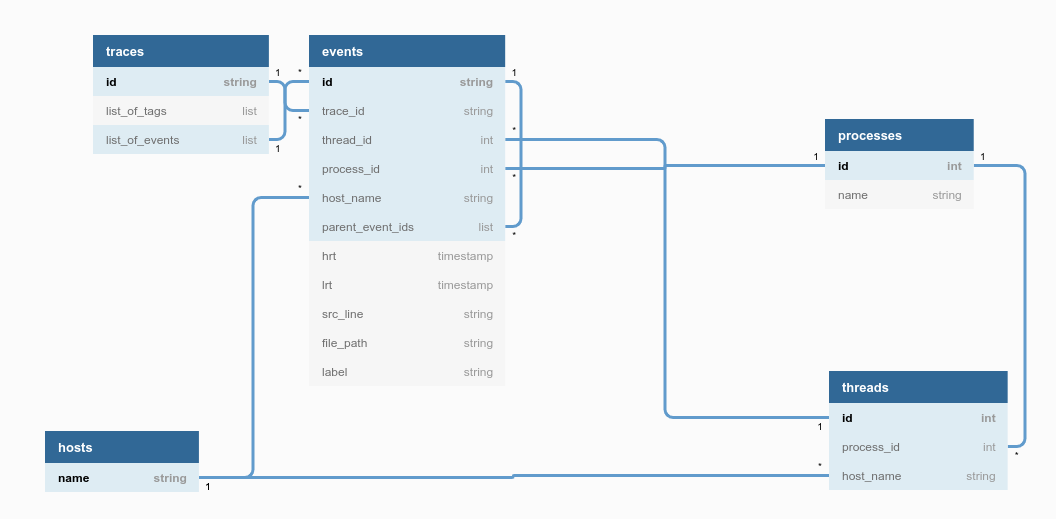
\includegraphics[width=\linewidth]{../data_abstractions.png}
    \caption{The different entities in TraViz.}
    \label{fig:entities}
  \end{figure}

\subsection{Trace}

A trace is a collection of events. It represents a request from a client to a service and shows the path of the
request through the microservice. A trace has three attributes: \textit{id}, \textit{list\_of\_tags}, and \textit{list\_of\_events}.
The \textit{id} of the trace is a categorical attribute used to identify a trace. The \textit{list\_of\_tags} is a list of human defined keywords that serve as
the metadata for the trace. There are on average two tags per trace in both datasets, but the socialNetwork
dataset has a total of 8 different tags and the HDFS dataset has a total of 22285 different tags. The
\textit{list\_of\_events} attribute is a list of the events that happened in a trace. The events in the list
are ordered, with events that caused another event preceding the caused event in the list. The causal relationship
between the events forms a DAG. There are around 100 events per trace in the socialNetwork dataset and 1400 events per trace
in the HDFS dataset.

\subsection{Event}

Events are important things that happen in a system, such as acquiring a lock, sending a request to another server,
or performing an update. In short, events are anything a developer things is useful enough to log. Events have 11
different attributes. They are \textit{id}, \textit{trace\_id}, \textit{thread\_id}, \textit{process\_id}, \textit{host\_name},
\textit{parent\_event\_ids}, \textit{hrt}, \textit{lrt}, \textit{src\_line}, \textit{file\_path}, and \textit{label}. The
\textit{id} is a categorical variable used to uniquely identify an event. The \textit{trace\_id} is another categorical
attribute that indentifies the trace that holds an event. The \textit{thread\_id} is a categorical variable that identifies the
thread that executed the event. The \textit{process\_id} gives the id of the process holding the thread that executed the event.
The \textit{host\_name} gives the name of the machine running the process that executed the event. An event can have at most one
host. The \textit{parent\_event\_ids} attribute is a collection of event ids. Each id maps to a parent event. The ids are used to
create a causal ordering between events. The socialNetwork and HDFS datasets have on average one parent event id per event, but 
can have up to two parent events for one event. 

The \textit{hrt} is a quantitative attribute that stands for high resolution time
stamp, and provides nanosecond level precision for the time an event was initiated. The \textit{lrt} is also a quantitative attribute.
It provides a milisecond level precision low resolution time stamp for the time an event occured. The \textit{src\_line} gives the line
in the source code where an event was logged. The \textit{file\_path} is a categorical attribute that gives the path to the file where 
a programmer logged this specific event. This attribute can be used with the \textit{src\_line} to find the exact line of code of a logged event.
The last attribute in an event is the \textit{label}. The label is a free-form text annotaion that gives a high-level description of the
event. Labels are a meaningful human added annotation for debugging, and there are 2,472 labels in the socialNetwork dataset and 210,957 labels
in the HDFS dataset.

\subsection{Host}

A host represents a node in the distributed system. Hosts encapsulate the processes and threads
that execute the events in a trace. There are 13 different hosts across the social network dataset
and 9 different hosts across the HDFS dataset. The host is identified by a categorical \textit{name} attribute , which is
referenced by events and threads.

\subsection{Process}

The process entity represents a operating system process running on
a host. Processes have a categorical \textit{id} attribute, which is referenced by the events and threads executed in
the process. The process also has a categorical \textit{name} attribute, which gives a human understandable name for the
application running the process. There are around 20 different processes per trace in the socialNetwork
dataset and 18 different processes per trace in the HDFS dataset. There are 13 different process names
in the socialNetwork dataset and 4 different process names in the HDFS dataset.

\subsection{Thread}

The thread entity represents
a kernel or user thread. Distinguishing between both is not important for the purposes of this project, so we
simply see it as the basic unit of execution. Threads have a categorical \textit{id} attribute that identifies a thread
within a trace. Events use the \textit{id} to signal the thread that executed them. It is important to note
that the thread \textit{id} does not match across traces, and the total number of threads is not useful because it's
not possible to correlate them between traces. Each thread also has two more categorical attributes: the \textit{host\_name}
and \textit{process\_id}. These attributes are used to identify the host and process that executed a thread. 

\section{Task Abstraction}

We have identified a total of six tasks that we want to support with our viz tool.
We discuss each task in detail with an example scenario below.

The first main task for this project is comparison. Namely, we want to compare the path and performance of different
requests. Each one of our traces represents a request and the collection of events in one trace forms a directed acyclic graph. Our
comparison tasks are meant to compare the structure of the DAGs created by the events and the duration of different requests. 
We want to support three different comparison tasks: one trace against one trace, one trace against many traces, and many traces
against many traces. In more abstract terms, we will compare the DAGs formed by the events in different traces by partitioning them
into side-by-side views or by showing some sort of a graph diff.

The second major task we are proposing is summarizing data. Many of the traces in our datasets are similar, so we want to
aggregate traces with the same tags and events. We believe aggregating traces with the same tags or events will give the user
a more generalized understanding of the traces. The user will be able to analyze the average duration of a group of traces, instead
of relying on the data from one single trace. This task will take the DAGs formed by the events of different traces and will summarize
them by aggregating traces with the same tags or events, so that we can better understand the topology and paths of these graphs.

There are two more tasks we want to support, but may be out of scope for the project so we are leaving these tasks as stretch goals.
The first task is creating a dependency graph using
the processes in a trace and the second task is adding source code integration to our tool. The \textit{process\_name} attribute in 
our dataset gives the name of a service in a microservice.
Developers building distributed systems are interested in understanding the structure of the microservice
architecture they are building. We want to consume the list of events in a trace and use the \textit{process\_name} attribute in an 
event to build a graph that links processes that trigger other processes. This information will be presented to developers so that 
they can discover the dependencies that build their microservices. 
The second task consists of using the \textit{src\_line} and \textit{file\_path}
attributes to locate the line in the source code that triggered an event. We will do this by providing a hyperlink to the file and line
in the github repository. 

\textbf{Scenario 1}: A developer wants to find out why two similar requests have very different 
completion times. The developer will select the two traces corresponding to the requests. After the traces are selected, our tool will
use the events of these traces to generate a view showing the differences between the traces as well as showing the
context and timing of the original requests. This will allow the developer to analyze and identify why 2 similar requests have 
different completion times.

 \textbf{Scenario 2}: A developer wants to find out why requests on Monday are
slower than the requests on Tuesday. The developer will make 2 different selections - selection of traces from Monday and selection
of traces from Tuesday. Our tool will aggregate the 2 selections into representative graphs and then show the difference of these
two aggregate traces. This will allow the developer to possibly figure out a high-level change between the request execution from
Monday to Tuesday.

 \textbf{Scenario 3}: A developer wants to analyze why a given trace is anomalous as compared to some of the previous
traces. To do this, the developer will first create a selection of traces that will be aggregated down into 1 trace. The developer
will then select the anomalous trace and create a comparison between the anomalous and the representative trace.
Our tool will show the difference between the 2 traces and allow the developer to figure out why a particular trace is anomalous.

 \textbf{Scenario 4}: A developer wants to understand the communication load between different services of the system.
Our tool will show the developer an overview graph that shows how often 2 services in the distributed system communicate
with each other. This will allow the developer to figure out how an addition of a new service would increase the load on each
service.

\section{Scenario}

\section{Solution}

Traviz accomplishes six tasks. These tasks are finding outliers and overviewing the dataset,
integrating source code and tracing data, extracting a detailed view of an individual trace, analyzing the
dependencies between the services in a distrbuted system, comparing two traces, and aggregating multiple traces
into a single visualization. Our solution to each one of these tasks is described in the subsections below.

\subsection{Outliers and Overview}

For this task we consume a set of traces and identify outliers and patterns.
We provide a visual representation of the distribution of the number of events in a trace, trace duration,
and date of a trace. We achieve this by
using crossfilter to display the distributions in a bar chart and arranging the tracing data in a table.

To reduce the cognitive load on the user, we reduce the number of items on display by using crossfilter
to select areas in the distribution charts, which causes the data table to be filtered accordingly. For example,
if a user selects the area between 1000ms and 2000ms in the latency distribution chart, the table will only display
traces that have a duration between 1000ms and 2000ms. The table can also be sorted to help users quickly find traces.
Visually representing the distributions in bar charts and filtering the data from these distributions allows users to swiftly
find outliers. For example, traces with more events than usual can be quickly identified from the bar chart and selected using our
filtering functionality.

\begin{center}
    \begin{tabular}{|p{.95\columnwidth}|}
        \hline
        \textbf{Outliers and Overview}                             \\
        \hline
        \textbf{What: data}                                        \\
        - A collection of traces                                   \\
        \hline
        \textbf{Why: tasks}                                        \\
        - Find outliers                                            \\
        - Identify patterns                                        \\
        \hline
        \textbf{How: reduce}                                       \\
        - Filter items using attributes such as number of events, duration,
        and date of a trace.                                       \\
        \textbf{How: show}                                         \\
        - Display traces on table that can be sorted and filtered. \\
        \hline
    \end{tabular}
\end{center}



\subsection{Source Code Integration}

Our source code integration tool consumes traces and derives the number of events
triggered by a line in the source code. This tool is useful at identifying what files - and lines in the source code of that file -
produce the most events. Developers can use the source code integration tool to identify what areas of their code are heavily utilized.

Our source code integration tool uses two bar charts to encode the relevant information. One of the charts aggregates the total number of events in a
file and displays one bar per file. If a user clicks on the bar for one of the files, Traviz displays another bar chart adjacent to it that
reveals the number of events in each source code line of the file. In both charts, we encode the number of events with the lenth and luminance
of the bar, where higher luminance means that more events spawned from that file or source code line. To complete the
source code integration, Traviz allows users to click on a bar in the source code line chart. A mouse click causes the application to
redirect the user to the line in a Github repo hosting the project being visualized.

\begin{center}
    \begin{tabular}{|p{.95\columnwidth}|}
        \hline
        \textbf{Source Code Integration}                                 \\
        \hline
        \textbf{What: data}                                              \\
        - A collection of traces                                         \\
        \hline
        \textbf{Why: tasks}                                              \\
        - Identify what files produce events                             \\
        - Identify what lines in a file produce the most or least events \\
        \hline
        \textbf{How: display}                                            \\
        - Display number of events in a file and number of events originating from a
        line in the source code using bar charts                         \\
        \textbf{How : encode}                                            \\
        - Encode number of events in a file and number of events originating from a line in the source code using the
        size of the bar.                                                 \\
        - Encode number of events in a file and number of events originating from a line in the source code using the
        luminance of the bar.                                            \\
        \hline
    \end{tabular}
\end{center}


\subsection{Individual Trace Analysis}

The individual trace analysis tool complements the overview tool and allows the details of a specific trace to be analysed.
This tool displays the timestamp of the events in a trace,
the thread where an event was executed, and the events that originated events in other threads. This tool is useful for a distributed systems
developer because it allows a trace to be dissected, so that the path of a request can be observed. The individual trace analysis tool
encodes each thread as a a lane, the time of an event as the position on the x-axis, and the thread of an event as the position on the y-axis. Furtermore,
if an event triggered an event in another thread, we show this relationship with a connecting line.

\begin{center}
    \begin{tabular}{|p{.95\columnwidth}|}
        \hline
        \textbf{Individual Trace Analysis}                                              \\
        \hline
        \textbf{What: data}                                                             \\
        - One trace                                                                     \\
        \hline
        \textbf{Why: tasks}                                                             \\
        - Observe the timing of events in a trace                                       \\
        - Identify events that triggered events in other threads                        \\
        \hline
        \textbf{How: encode}                                                            \\
        - Encode each thread as a lane                                                  \\
        - Encode the time of an event as the position of a point on the x-axis          \\
        - Encode the thread of an event as the position of a point on the y-axis        \\
        - Identify events that triggered events in other threads with a connecting line \\
        \hline
    \end{tabular}
\end{center}


\subsection{Service Dependency Analysis}


The service dependency analysis derives the total number of messages issued by a service.
This tool is important for comprehending distributed systems because it allows developers to understand the
dependency relationship between services. For example, in a micro-service architecture, the dependency graph helps understand what services
talk to each other and what services talk to the most services. To visualize the dependencies, we arranged the services into
a node-link graph, where each service is a node, and the dependency is a link between the nodes. We also encoded the degree of each node as the area of
a circle, so that services that talk to many services can be easily recognized.

\begin{center}
    \begin{tabular}{|p{.95\columnwidth}|}
        \hline
        \textbf{Service Dependency Analysis}                                   \\
        \hline
        \textbf{What: derived data}                                            \\
        - Total messages issued by a service                                   \\
        \hline
        \textbf{Why: task}                                                     \\
        - Understand the dependency between services                           \\
        \hline
        \textbf{How: arrange}                                                  \\
        - Arrange services into a node-link graph                              \\
        - Services are represented as nodes                                    \\
        - Dependencies between services are represented as links between nodes \\
        \textbf{How: encode}                                                   \\
        - Encode the amount of dependencies in a service with the area
        of the node                                                            \\
        \hline
    \end{tabular}
\end{center}


\subsection{Trace Comparison}

In this tool we take two traces and merge them in a way that the user can indentify the
differences and similarities between the traces. Understanding the differences and similarities
between a trace can help developers identify why some requests take longer than others.

To build this tool we assigned each event in both traces a group between 1 and 3. The events are arranged into a node-link graph,
where each event is a node and the link encodes the parent-child relationship between events. We encode group 3 nodes as squares and groups 1 and 2 as circles.
We also encode the group a node belongs to using hue. Group three nodes are grey, group one nodes are ----, and group two nodes are -----. We aggregate
group three nodes, with the intent of reducing the total number of nodes in the graph and reduce cognitive load. Users can disaggregate group three nodes if they
want to take a look at the full graph. If users want to look at the details of an event, they can click on a node, which causes the attributes of the selected event
to be displayed on the side.

\begin{center}
    \begin{tabular}{|p{.95\columnwidth}|}
        \hline
        \textbf{Trace Comparison}                                                           \\
        \hline
        \textbf{What: data}                                                                 \\
        - Two traces                                                                        \\
        \hline
        \textbf{Why: tasks}                                                                 \\
        - Identify differences between traces                                               \\
        - Observe patterns                                                                  \\
        \hline
        \textbf{How: arrange}                                                               \\
        - Arrange events into a node-link graph                                             \\
        - Events are represented as nodes                                                   \\
        - Parent-child relattionships between events are represented as links between nodes \\
        \textbf{How: encode}                                                                \\
        - Encode nodes in group 3 as squares and nodes in groups 1 and 2 as circles         \\
        - Encode the group of an event using hue                                            \\
        \textbf{How: aggregate}                                                             \\
        - Aggregate group 3 nodes to reduce the size of the graph                           \\
        \hline
    \end{tabular}
\end{center}


\subsection{Trace Aggregation}

The trace aggregation tool helps users see the big picture. It consumes a collection of traces and arranges
them into a node-link graph, where nodes represent events and links represent the parent-child relationships between
the events. To condense the information from multiple traces into a more manageable graph, we aggregate the events
from the same source code line into one node. We also visualize the number of events in a node by using luminance, where high
luminance means a node is responsible for many events, and low luminance means that a node is responsible for few events. A node can
be selected by clicking, which results in detailed information about that event - such as the event id, timestamp, and thread id - to be displayed.
The aggreagation tool also allows the structure from multiple traces to be analysed, while reducing the amount of nodes on display.

\begin{center}
    \begin{tabular}{|p{.95\columnwidth}|}
        \hline
        \textbf{Trace Aggregation}                                                          \\
        \hline
        \textbf{What: data}                                                                 \\
        - A collection of traces                                                            \\
        \hline
        \textbf{Why: tasks}                                                                 \\
        - Visualizing the big picture                                                       \\
        - Analyzing multiple traces                                                         \\
        \hline
        \textbf{How: arrange}                                                               \\
        - Arrange avents into a node-link graph                                             \\
        - Events are represented as nodes                                                   \\
        - Parent-child relattionships between events are represented as links between nodes \\
        \textbf{How: aggregate}                                                            \\
        - Aggregate events from the same source code line as one node                       \\
        \textbf{How: encode}                                                                \\
        - Encode number of events in a node with luminance                                  \\
        - High luminance means a node is aggregating many events                            \\
        - Low luminance means a node is aggregating few events                              \\
        \hline
    \end{tabular}
\end{center}


\section{Implementation Approach}

Our visualization tool will be a webapp. We will host a backend written in Go that 
will serve requests from a client. The frontend will be written in javascript. We will use D3 to manipulate the data served
by our backend and to create the visualizations necessary to fulfill our comparison tasks.

\section{Related Work}

\textbf{TODO: Add Related}

\balance
{\footnotesize
\bibliographystyle{abbrv}
\bibliography{report}
}

\end{document}

